\documentclass[a4]{article}

\usepackage[left=3cm,right=3cm,top=2cm,bottom=2cm]{geometry} 

\usepackage[utf8]{inputenc} 
\usepackage[           spanish % para poder usar el español
                      ,es-tabla % para los captions de las tablas
                       ]{babel}   
\decimalpoint

\usepackage[bookmarks=true,
            bookmarksnumbered=false, % true means bookmarks in 
                                     % left window are numbered
            bookmarksopen=false,     % true means only level 1
                                     % are displayed.
            colorlinks=true,
            linkcolor=blue,
            urlcolor=cyan]{hyperref}
            
\usepackage[T1]{fontenc}
\usepackage{lmodern}

\usepackage{parskip}
\usepackage{xcolor}

\usepackage{multirow}

\usepackage{amsmath,amssymb,amsthm}

\usepackage{caption}

\usepackage{listings}
\lstset
{ %Formatting for code in appendix
  language=C++, % choose the language of the code
  basicstyle=\fontfamily{pcr}\selectfont\footnotesize\color{black},
  keywordstyle=\color{darkorange}\bfseries, % style for keywords
  numbers=left, % where to put the line-numbers
  numberstyle=\tiny, % the size of the fonts that are used for the line-numbers     
  backgroundcolor=\color{white},
  showspaces=false, % show spaces adding particular underscores
  showstringspaces=false, % underline spaces within strings
  showtabs=false, % show tabs within strings adding particular underscores
  tabsize=2, % sets default tabsize to 2 spaces
  captionpos=b, % sets the caption-position to bottom
  breaklines=false, % sets automatic line breaking
  breakatwhitespace=false, 
}

\usepackage{enumerate}% paquete para poder personalizar fácilmente la apariencia de las listas enumerativas

\usepackage{graphicx} % figuras
\usepackage{subfigure} % subfiguras

\definecolor{darkorange}{rgb}{0.94,0.4,0.0}
	
\usepackage{float} % para controlar la situación de los entornos flotantes

\restylefloat{figure}
\restylefloat{table} 

\newcommand{\HRule}{\rule{\linewidth}{0.5mm}}

\author{David Cabezas Berrido}
\date{\vspace{-5mm}}

\title{\huge Práctica 4: Algoritmos Backtracking \\ y Branch \& Bound \HRule\vspace{-4mm}}

\setcounter{section}{-1}

\begin{document}
\maketitle
\vspace{20mm}
\tableofcontents

\newpage

\section{Problema}

Se celebra una cena de gala con $n$ invitados, cada invitado tendrá
sentados a dos comensales a su izquierda y a su derecha y conocemos la
afinidad que tiene cada invitado $i$ con cada invitado $j$. El nivel
de conveniencia total de una asignación es la suma de las afinidades
de cada invitado con las personas de su izquierda y derecha, Debemos
maximizar este valor.

\section{Algoritmo}

Usaremos la técnica de \textbf{Backtracking} para encontrar la
solución óptima al problema. Procederemos del siguiente modo:

\begin{itemize}
\item Sentamos a la persona 0 en el asiento 0 (por simplicidad).
\item Probamos todas las posibilidades de personas a sentar en el
  asiento 1.
\item Para cada una de estas posibilidades, probamos todas las
  posibilidades de personas a sentar en el asiento 2.
\item Procedemos hasta llenar la mesa, cada vez que sentamos a una
  persona sumamos la afinidad que genera a la afinidad de la
  configuración anterior.
\item Cada vez que completamos una configuración con $n$ personas, la
  guardamos como mejor solución si tiene más afinidad total que la
  mejor solución encontrada hasta el momento.
\end{itemize}

Este sería el algoritmo de fuerza bruta, que tiene complejidad
factorial ya que explora todas las permutaciones para sentar a las
$n-1$ personas restantes una vez fijada la persona 0. Este algoritmo
encuentra siempre la solución óptima, pero es muy costoso. Así que
utilizaremos la técnica de \textbf{Backtracking} para ahorrarnos
probar con varias de las combinaciones innecesariamente y así
encontrar la solución óptima en menor tiempo.

Si tenemos una configuración parcial con $k < n$ personas sentadas en
los sitios $0,\ldots,k-1$, el algoritmo de fuerza bruta probaría las
$n-k$ posibles personas para sentar en el sitio $k$, y con cada una de
estas configuraciones, $n-k-1$ posibles personas para sentar en el
sitio $k+1$\ldots.

Existe la posibilidad de que no encontremos ninguna solución mejor a
partir de esta solución parcial, y si lo supiéramos de antemano
podríamos ahorrarnos $(n-k)!$ llamadas a la función. Pues bien, sea
$A$ la afinidad de la configuración parcial. Para cada persona que
queda por sentarse calculamos las dos afinidades mayores que podría
tener y para las personas de los sitios 0 y $k-1$ la mayor afinidad
posible. Cualquier solución que desarrollemos a partir de esta
configuración parcial tendrá su afinidad acotada por este valor, por
lo que cuando este valor no supere la afinidad de la mejor solución
encontrada hasta el momento no encontraremos nada explorando esta
rama, luego ahorraremos las $(n-k)!$ llamadas recursivas.

De esta forma encontramos la solución óptima ahorrando probar varias
configuraciones innecesarias.

\subsection{Código}

\subsubsection{Cota de afinidad}

\begin{lstlisting}
  void mayoresAfinidades(int persona, int& max1, int& max2) const{
    max1 = max2 = 0;

    for(int j = 0; j < n; j++)
    if(afinidad[persona][j] > max1){
      max2 = max1;
      max1 = afinidad[persona][j];
    }
    else if(afinidad[persona][j] > max2)
      max2 = afinidad[persona][j];
  }
\end{lstlisting}
\begin{lstlisting}
  int cotaAfinidad(const vector<int> &sentados, int afActual) const{
    int maxA = afActual;
    int max1, max2;

    for(int i = 1; i < n; i++)
      if(find(sentados.begin(),sentados.end(),i)==sentados.end()){
        mayoresAfinidades(i,max1,max2);
        maxA += max1+max2; 
      }
   
    mayoresAfinidades(sentados.front(),max1,max2);
    maxA += max1;
    mayoresAfinidades(sentados.back(),max1,max2);
    maxA += max1;

    return maxA;
  }
\end{lstlisting}

\subsubsection{Función recursiva para probar las posibles configuraciones}

\begin{lstlisting}
  void backtracking(const Cena& cena, const vector<int> &sentados, vector<int> &bestSol,
                    int currentAffinity, int& bestAffinity){
    if(sentados.size() == cena.getN()){
      currentAffinity += cena.getAfinidad(sentados.back(),sentados.front())
                       + cena.getAfinidad(sentados.front(),sentados.back());
      if(currentAffinity > bestAffinity){
        bestAffinity = currentAffinity;
        bestSol = sentados;
      }
      return;
    }
    
    if(cena.cotaAfinidad(sentados, currentAffinity) <= bestAffinity){
      return;
    }
    
    int aff;
    vector<int> aux;
    
    for(int i = 1; i < cena.getN(); i++){
      aff = currentAffinity;
      aux = sentados;
      if(find(sentados.begin(),sentados.end(),i)==sentados.end()){
        aux.push_back(i);
        aff += cena.getAfinidad(i,sentados.back()) + cena.getAfinidad(sentados.back(),i);
        backtracking(cena, aux, bestSol, aff, bestAffinity);
      }
    }
  }
\end{lstlisting}

Sólo tenemos que sentar a la persona 0 en el asiento 0 y llamar a la
función. Opcionalmente podemos calcular una solución real cualquiera y
su afinidad e inicializar la mejor 

\subsection{Eficiencia}

La eficiencia teórica de este algoritmo sigue siendo factorial, ya que
en el peor de los casos no se ahorran llamadas a la función (la cota
siempre es mayor que la mejor solución hasta el momento). No obstante,
en la práctica sí que se ahorran llamadas recursivas, por lo que el
tiempo de ejecución es mucho menor.

\newpage

\section{Resultados Empíricos}

He realizado varias simulaciones y calculado el tiempos medio de
ejecución de los algoritmos \textbf{Backtracking} y \textbf{Fuerza
  Bruta} para varios ejemplos aleatorios con distinto número de
comensales. En la siguiente tabla se aprecia la mejora en el
tiempo de ejecución que supone el \textbf{Backtracking}.

\begin{figure}[!hbp]
  \centering
  \label{tab:tiempos}
  \begin{tabular}{| c | c | c | c |}
    \hline
    \multicolumn{1}{|c|}{$\textbf{n}$}& \textbf{Backtracking}&
    \textbf{Fuerza Bruta}& \textbf{Ganancia} \\ \hline
     3 & 1.81e-05  & 2.28e-05  & 1.259669  \\ 
     4 & 6.68e-05  & 1.49e-05  & 0.223054  \\ 
     5 & 7.02e-05  & 6.38e-05  & 0.908832  \\ 
     6 & 0.0003676 & 0.0003573 & 0.971980  \\ 
     7 & 0.0017335 & 0.0020342 & 1.173464  \\ 
     8 & 0.0070328 & 0.014561  & 2.070441  \\ 
     9 & 0.028686  & 0.128955  & 4.495398  \\ 
    10 & 0.170039  & 1.27693   & 7.509630  \\ 
    11 & 0.950164  & 13.8355   & 14.561170 \\ 
    12 & 2.99369   & 165.75    & 55.366454 \\ \hline
  \end{tabular}
\end{figure}

\subsection{Gráficas}

En la gráfica de la izquierda se aprecia el crecimiento del tiempo de
ejecución del algoritmo, similar al de la función factorial. En la
gráfica de la derecha destaca su eficiencia en comparación con el de
fuerza bruta.

\begin{figure}[H]
  \centering
  \subfigure[Algoritmo Backtracking]{\label{graf:backtracking}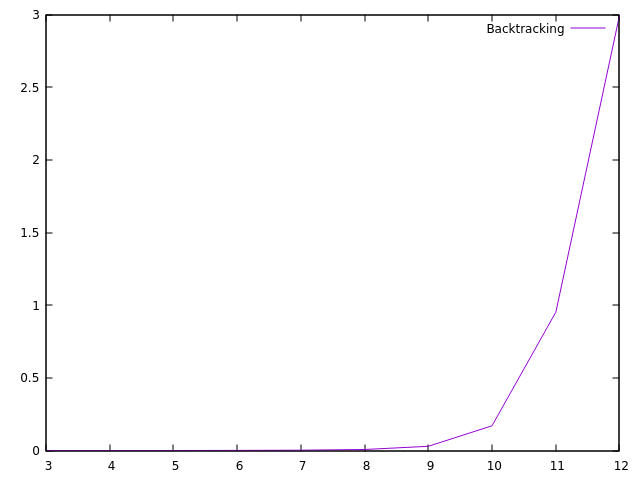
\includegraphics[width=77mm]{graficas/backtracking}}
  \subfigure[Comparación con algoritmo de fuerza bruta]{\label{graf:comparacion}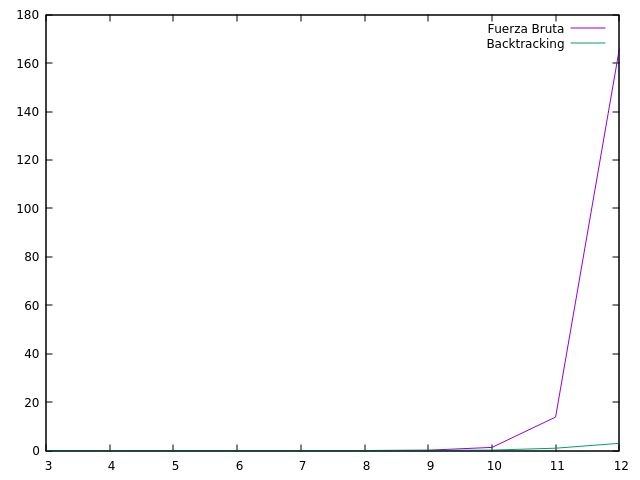
\includegraphics[width=77mm]{graficas/comparacion}}
\end{figure}

\section{Conclusión}

En esta práctica, he comprobado cómo la tecnica de Backtracking puede
hallar la solución óptima a un problema en un tiempo mucho menor que
el algoritmo de fuerza bruta por medio de evitar comprobaciones
innecesarias.

\end{document}